% preamble;
\documentclass[11pt]{article}
\usepackage[a4paper, 
			left=1.5in,
			right=1.5in,
			top=1.5in,
			bottom=1.5in]{geometry}
% \linespread{1.25} 

%%% PACKAGES

% A packages
\usepackage{adjustbox}
\usepackage{afterpage}
\usepackage{authblk}
\usepackage{amsmath}
\usepackage{amssymb}
\usepackage{amsfonts}
\usepackage{amsthm}
\usepackage{appendix}


% B packages
\usepackage{booktabs}
\usepackage{blindtext}
\usepackage[style=apa, sortcites,backend=biber,giveninits=true]{biblatex}
\usepackage[english]{babel}


% C packages
\usepackage{caption}
\usepackage{color}


% E packages
\usepackage{enumerate}
\usepackage{epigraph}

% F packages
\usepackage{footmisc}
\usepackage[T1]{fontenc}
\usepackage{float}
\usepackage{fullpage}

% G packages
\usepackage{graphicx}
\usepackage{geometry}

% H packages
\usepackage[colorlinks=true,linkcolor=blue, citecolor=blue]{hyperref}


% I packages
\usepackage[utf8]{inputenc}
\usepackage{csquotes}

% L packages
\usepackage{longtable}
\usepackage{lscape}
\usepackage{ltablex}

% M packages
\usepackage{multirow}
\usepackage{multicol}

% N packages

% O packages
\usepackage{optidef}

% P packages
\usepackage{pbox}

% R packages
\usepackage{ragged2e}
\usepackage{rotating}
\usepackage{relsize}


% S packages
\usepackage[onehalfspacing]{setspace}
\usepackage{siunitx}
\usepackage[lofdepth]{subfig}


% T packages
\usepackage{tabularx}
\usepackage{titlesec}

% U packages
\usepackage{url}
\renewcommand{\UrlFont}{\footnotesize}

% V packages
\usepackage{verbatim}

% X packages
\usepackage{xfrac}
\usepackage{xpatch}

% Other comands
\newtheorem{proposition}{Proposition}
\newtheorem{assumption}{Assumption}
\newtheorem{definition}{Definition}
\newtheorem{solution}{Solution}
\newtheorem{theorem}{Theorem}
\newtheorem{lemma}{Lemma}
\newcolumntype{C}[1]{>{\centering}m{#1}}




%%% PREAMBLE TO GENERATE NICE ESTOUT STATA TABLES
%%% http://www.jwe.cc/2012/03/stata-latex-tables-estout/

% *****************************************************************
% Estout related things
% *****************************************************************
\newcommand{\sym}[1]{\rlap{#1}}% Thanks to David Carlisle

\let\estinput=\input% define a new input command so that we can still flatten the document

\newcommand{\estwide}[3]{
	\vspace{0.3cm}{
		\begin{tabular*}
			{\textwidth}{@{\hskip\tabcolsep\extracolsep\fill}l*{#2}{#3}}
			\hline\hline
			\addlinespace[0.3cm]
			\estinput{#1}
			\hline\hline
			\addlinespace[0.3cm]
		\end{tabular*}
	}
}	

\newcommand{\estauto}[3]{
	\vspace{0.3cm}{
		\begin{tabular}{l*{#2}{#3}}
			\hline\hline
			\addlinespace[0.3cm]
			\estinput{#1}
			\hline\hline
			\addlinespace[0.3cm]
		\end{tabular}
	}
}

% Allow line breaks with \\ in specialcells
\newcommand{\specialcell}[2][c]{%
	\begin{tabular}[#1]{@{}c@{}}#2\end{tabular}}

% *****************************************************************
% Custom subcaptions
% *****************************************************************
% Note/Source/Text after Tables
\newcommand{\figtext}[1]{
	%\vspace{-1.9ex}
	\captionsetup{justification=justified,font=footnotesize}
	\caption*{\hspace{0pt}\hangindent=0.0em #1}
}
\newcommand{\fignote}[1]{\figtext{\emph{Note:~}~#1}}

\newcommand{\figsource}[1]{\figtext{\emph{Source:~}~#1}}

% Add significance note with \starnote
\newcommand{\starnote}{\figtext{* p < 0.1, ** p < 0.05, *** p < 0.01. Standard errors in parentheses.}}

% *****************************************************************
% siunitx
% *****************************************************************
\sisetup{
	detect-mode,
	tight-spacing		= true,
	group-digits		= false ,
	input-signs		= ,
	input-symbols		= ( ) [ ] - + *,
	input-open-uncertainty	= ,
	input-close-uncertainty	= ,
	table-align-text-post	= false
}

% style;
% \usepackage{mathpazo}

% bibliography command;
\addbibresource{bibliography/bibliography.bib}

% header;
\title{Title\thanks{Many thanks to everyone.}}
\author{Ahmad A. Mourad Jr.\footnote{ahmad.mourad16@gmail.com}}

\begin{document}
\maketitle

% abstract;
\begin{abstract}
In this document, I draw a paper template that anyone can use for any purposes, with a complete preamble including features of Stata to \LaTeX automated tables and so on.
\end{abstract}

\textit{Keywords}:

\textit{JEL Codes}:

% table of contents;
\tableofcontents

% data construction;
\section{Introduction}

\subsection{Related Literature}

You can cite your references using \textcite{amihud2002illiquidity}, or using \parencite{amihud2002illiquidity} or even \cite{amihud2002illiquidity}. It also works for \textcite{eugene1992cross} and \textcite{novy2013other}. You can also use (\cite{amihud2002illiquidity} and \cite{novy2013other}).





















% data;
\section{Data}

For summary statistics, see Table \ref{tab:table1}. To access R\&D expenses in 2012, see Figure \ref{fig:fig1}.

\begin{center}
    [Table \ref{tab:table1} and Figure \ref{fig:fig1} here]
\end{center}











% results;
\section{Results}

Regression specification is as follows:
\begin{equation}
    \label{reg:reg1}
    y_{it} = a_i + x_{it}^{\prime} \beta + \epsilon_{it}
\end{equation}

For panel regression results on Total Dividends and Net Income on a set of control variable, as in equation \ref{reg:reg1}, see Table \ref{tab:table2}.

\begin{center}
    [Table \ref{tab:table2} here]
\end{center}


% conclusion;
\section{Conclusion}
A section for a bunch of nice conclusions.


% references;
\addcontentsline{toc}{section}{References}
\printbibliography

% new page;
\newpage

% appendix;
\appendix
\section{Figures}

\begin{figure}[htbp]
\centering
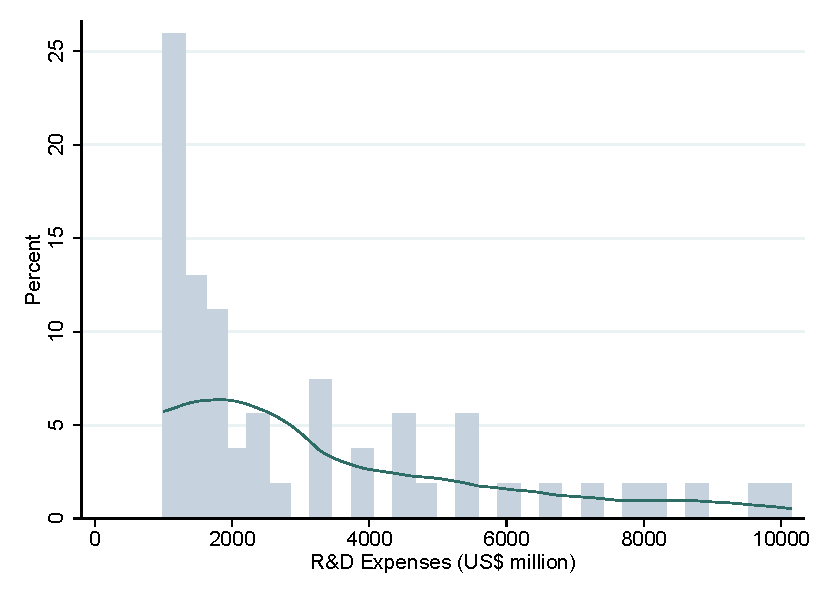
\includegraphics{figures/histogram_rd.pdf}
\caption{Distribution of R\&D expenses for US firms in 2012.}
\label{fig:fig1}
\end{figure}

\section{Tables}

\begin{table*}[htbp]
\small 
\caption{\label{tab:table1} Summary Statistics}
\adjustbox{max width=\textwidth}{
\estwide{tables/summary_statistics.tex}{8}{S[table-format=2.2]}
}
\figtext{Summary statistics for Market Value of Equity, Book Value of Equity, Book-to-Market Ratio and Leverage for US firms between 2010 and 2019. Values of Market Value of Equity, Book Value of Equity are expressed in US\$ millions.}
\end{table*}


\begin{table*}[htbp]
\small 
\caption{\label{tab:table2} Panel Regressions}
\adjustbox{max width=\textwidth}{
\estwide{tables/regressions.tex}{8}{S[table-format=2.2]}
}
\figtext{\footnotesize This table shows panel regressions for Net Income and Total Dividends on a set of control lagged variables. $R\&D$ stands for research and development expenses on lagged periods, $MarketEquity$ stands for the market equity value of the firm, $BM$ stands for the book-to-market ratio and $IndustryShare$ stands for the within input share for each industry. Standard errors are robust to heteroskedasticity, p-values are in parenthesis with *** $p < 0.01$, ** $p < 0.5$, * $p < 0.1$.}
\end{table*}

\end{document}


